\documentclass[twocolumn]{IEEEtran}
\usepackage{graphicx}
\usepackage[utf8x]{inputenc}
\usepackage{times}
\usepackage{amssymb,amsfonts}
\usepackage[tbtags]{amsmath}
\usepackage{cite}
\usepackage{slashbox}
\usepackage{pict2e}
\usepackage{float}
\usepackage[all]{xy}
\usepackage{graphics,graphicx,color,colortbl}
\usepackage{times}
\usepackage{subfigure}
\usepackage{wrapfig}
\usepackage{multicol}
\usepackage{cite}
\usepackage{url}
\usepackage[tbtags]{amsmath}
\usepackage{amsmath,amssymb,amsfonts,amsbsy}
\usepackage{bm}
\usepackage{algorithm}
\usepackage{algorithmic}
\usepackage[centerlast, small]{caption}
\usepackage[colorlinks=true, citecolor=blue, linkcolor=blue, urlcolor=blue,
breaklinks=true]{hyperref}

\begin{document}
\title{Análisis de Nodos, Mallas y Teorema de Superposición}
\author{José Fabio Lozano Ovalle Código: $222982$\\
	Wilson Orlando Macias Fuquen Código: $223101$\\
	David Ricardo Martínez Hernández Código: $261931$}
\maketitle
\markboth{Universidad Nacional de Colombia}{}
\floatname{algorithm}{Algoritmo}

\begin{abstract}
Utilizando arreglos de resistencias, en estrella y triangulo, se construirán diferentes  circuitos para comprobar experimentalmente las técnicas de análisis de mallas y nodales, también usando  varias fuentes DC y AC se realizará un análisis del teorema de superposición.
\end{abstract}

\begin{keywords}
Nodo, Lazo, Rama, Circuito lineal
\end{keywords}

\section{Objetivos}
\begin{itemize}
 \item Comprende y comprobar experimentalmente las diferentes técnicas de análisis de circuitos.
 \item Emplear el principio del teorema de superposición para resolver un circuito con dos o más fuentes.
 \item Reconocer la diferencia entre los modelos teóricos y los modelos prácticos de los elementos que componen un circuito.
\end{itemize}

\section{Introducción}
\noindent
Existen $2$ métodos básicos para realizar el análisis de circuitos eléctricos, las cuales se derivan de las leyes de Kirchhoff, estas leyes son: \textbf{Ley de corrientes} y \textbf{Ley de voltajes} (Nodos y Mallas). Existe a demás un teorema que facilita el análisis sobre los elementos de un circuito lineal que contiene $2$ o mas fuentes; pueden ser de voltaje o de corriente, este método se le conoce como el \textbf{Teorema de Superposición}.

\section{Marco Teórico}
\noindent
\textbf{Nodo}: Es un punto en el cual dos o mas elementos tiene una conexión común.\\
\textbf{Lazo}: Es una trayectoria cerrada la cual comienza y termina en el mismo nodo.\\
\textbf{Rama}: Es una trayectoria única en una red, compuesta por un elemento simple y el nodo en cada extremo de ese elemento.\\
\textbf{Circuito lineal}: Es aquel que esta compuesto en forma completa de fuentes independientes, fuentes dependientes lineales y elementos lineales.\\

\subsection{Teorema de Superposición}
\noindent
En cualquier red resistiva lineal, la tensión o la corriente a través de cualquier resistor o fuente se calcula sumando algebraicamente todas la tensiones o corrientes individuales ocasionadas por fuentes independientes separadas que actúan solas, junto con todas las demás fuentes de tensión independientes sustituidas por cortocircuitos y todas las demás fuentes de corriente independientes, sustituidas por circuitos abiertos.
\begin{figure}[H]
	\centering
		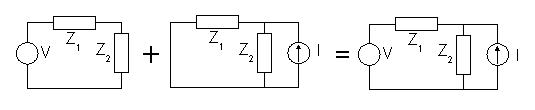
\includegraphics[scale=0.5]{ejemplo.png}
	\caption{Ejemplo de Superposición}
	\label{fig20}
\end{figure}

\subsection{Ley de corrientes de Kirchhoff}
\noindent
En cualquier nodo la suma de todas las corrientes que entran a ese nodo es igual a la suma de todas las corrientes que salen, o también la suma algebraica de las corrientes que llegan  aun nodo es cero.
\begin{equation}
 \sum\limits_{k = 1}^n {{l_k} = {I_1} + {I_2} + {I_3}... + {I_n} = 0} 
\label{equ1}
\end{equation}
\begin{figure}[H]
	\centering
		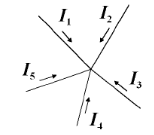
\includegraphics[scale=0.7]{n1.png}
	\caption{Ejemplo de Ley de corrientes de Kirchhoff}
	\label{fig21}
\end{figure}
\noindent
\begin{equation}
 {I_1} + {I_2} + {I_3} + {I_4} + {I_5} = 0
\end{equation}

\subsection{Ley de tensiones de Kirchhoff}
\noindent
En cualquier trayectoria cerrada de corriente la sumatoria de todas las caídas de tensión  es igual a la tensión total suministrada, o también la suma algebraica de las tensiones alrededor de cualquier trayectoria cerrada es cero.
\begin{equation}
 \mathop \sum \limits_{k = 1}^n {V_k} = {V_1} + {V_2} + {V_3} \ldots  + {V_n} = 0
\end{equation}
\begin{figure}[H]
	\centering
		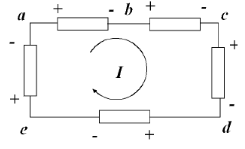
\includegraphics[scale=0.7]{v1.png}
	\caption{Ejemplo de Ley de voltajes de Kirchhoff}
	\label{fig22}
\end{figure}
\begin{equation}
 \left( {{V_a} - {V_b}} \right) + \left( {{V_b} - {V_c}} \right) + \left( {{V_c} - {V_d}} \right) + \left( {{V_d} - {V_e}} \right) + \left( {{V_e} - {V_a}} \right) = 0
\end{equation}

\section{Hipótesis}
\noindent
Al analizar un circuito por mallas o nodos y resolverlo nuevamente por superposición se deben obtener datos aproximadamente iguales,  además los datos obtenidos teóricamente deben ser aproximados al datos que se toman experimentalmente.\\
Cuando se  analiza un circuito de alta frecuencia, en la teoría no afecta el análisis, en la práctica esto puede afectar los elementos de medición ya estos tienen limitaciones respecto a esta característica y las mediciones pueden variar.

\section{Materiales}
\begin{itemize}
 \item Cables
 \item Conectores
 \item Fuente dual
 \item Generador de señales
 \item Multímetros
 \item Osciloscopio
 \item Pinzas
 \item Resistencias
\end{itemize}

\section{Análisis y Resultados Teóricos}
\noindent
Se realizo el análisis al circuito de la FIg. \ref{fig1}
\begin{figure}[H]
	\centering
		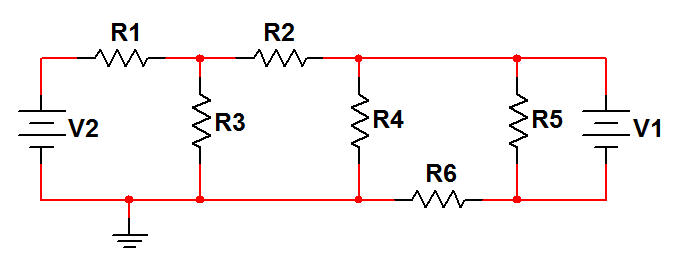
\includegraphics[scale=0.5]{m1.png}
	\caption{Circuito con dos fuentes}
	\label{fig1}
\end{figure}
\noindent
$R_1=R_4=1\ K \Omega$, $R_2=2.2 \ K \Omega$, $R_3=10 \ K \Omega$, $R_5= 100 \ \Omega$ Y $R_6 = 120 \ \Omega$

\subsection{Análisis por Kirchhoff}
\noindent
Las ecuaciones que se obtuvieron al analizarlo por Kirchhoff se obtuvieron las siguientes ecuaciones de malla
\begin{equation}
 {V_2} = {I_1}\left( {{R_1} + {R_3}} \right) - {I_2}{R_3}
\label{ecu1}
\end{equation}

\begin{equation}
 0 =  - {I_1}{R_3} + {I_2}\left( {{R_2} + {R_3} + {R_4}} \right) - {I_3}{R_4}
\label{ecu2}
\end{equation}

\begin{equation}
 0 =  - {I_2}{R_4} + {I_3}\left( {{R_4} + {R_5} + {R_6}} \right) - {I_4}{R_5}
\label{ecu3}
\end{equation}

\begin{equation}
 {V_1} = {I_4}{R_5}
\label{ecu4}
\end{equation}
\noindent
De la ecu. (\ref{ecu4}) se puede deducir que $I_4 = \frac{V_1}{R_5} = 0.05 \ mA$, por consiguiente la matriz queda como la ecu. (\ref{ecu5})
\begin{equation}
\footnotesize
\left[ {\begin{array}{*{20}{c}}
   {{R_1} + {R_3}} & { - {R_3}} & 0  \\
   {{R_3}} & {{R_2} + {R_3} + {R_4}} & { - {R_4}}  \\
   0 & { - {R_4}} & {{R_4} + {R_5} + {R_6}}  \\
\end{array}} \right]\left[ \begin{array}{l}
 {I_1} \\ 
 {I_2} \\ 
 {I_3} \\ 
 \end{array} \right] = \left[ \begin{array}{l}
 {V_2} \\ 
 0 \\ 
 V_{R_5} \\ 
 \end{array} \right]
\label{ecu5}
\end{equation}
\noindent
Siendo la ecu. (\ref{ecu6}) la matriz resultado
\begin{equation}
\footnotesize
 \left[ \begin{array}{l}
 {I_1} \\ 
 {I_2} \\ 
 {I_3} \\ 
 \end{array} \right] = {\left[ {\begin{array}{*{20}{c}}
   {{R_1} + {R_3}} & { - {R_3}} & 0  \\
   {{R_3}} & {{R_2} + {R_3} + {R_4}} & { - {R_4}}  \\
   0 & { - {R_4}} & {{R_4} + {R_5} + {R_6}}  \\
\end{array}} \right]^{ - 1}}\left[ \begin{array}{l}
 {V_2} \\ 
 0 \\ 
 V_{R_5} \\ 
 \end{array} \right]
\label{ecu6}
\end{equation}
\noindent
Por consiguiente el valor de las corriente se encuentra en la siguiente matriz ecu. \ref{ecu7}
\begin{equation}
\left[ \begin{array}{l}
 {I_1} \\ 
 {I_2} \\ 
 {I_3} \\ 
 \end{array} \right] = \left[ \begin{array}{l}
 9.686 \ mA\\ 
 8.155 \ mA\\ 
 10.782 \ mA\\ 
 \end{array} \right]
\label{ecu7}
\end{equation}
\noindent
Los voltajes teóricos son:

\begin{table}[H]
	\centering
\begin{tabular}[c]{|c|c|c|c|c|c|} \hline
$V_{R_1}$ & $V_{R_2}$ & $V_{R_3}$ & $V_{R_4}$ & $V_{R_5}$ & $V_{R_6}$ \\ \hline
$9.686$ & $17.9412$ & $15.313$ & $2.627$ & $5$ & $1.293$ \\ \hline
\end{tabular}
	\caption{Voltajes obtenidos teóricamente}
	\label{tab1}
\end{table}

\subsection{Análisis por Superposición}
\noindent
Las ecuaciones de superposición que se obtuvieron fueron las siguientes:\\
$$V_2 = 0$$
\begin{figure}[H]
	\centering
		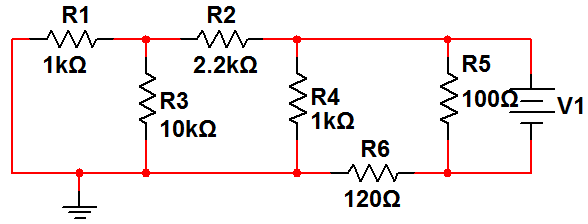
\includegraphics[scale=0.45]{c1.png}
	\caption{Fuente $V_2$ a cero}
	\label{fig2}
\end{figure}
\noindent
Las ecuaciones para este circuito son las siguientes:
\begin{equation}
 0 = {I_{1a}}\left( {{R_1} + {R_3}} \right) - {I_{2a}}{R_3}
\end{equation}
\begin{equation}
 0 =  - {I_{1a}}{R_3} + {I_{2a}}\left( {{R_2} + {R_3} + {R_4}} \right) - {I_{3a}}{R_4}
\end{equation}
\begin{equation}
 {V_1} =  - {I_{2a}}{R_4} + {I_{3a}}\left( {{R_4} + {R_5} + {R_6}} \right) - {I_{4a}}{R_5}
\end{equation}
\noindent
Dado que $I_{4a} = \frac{V_1}{R_5} = 0.05 \ mA$
\begin{equation}
\footnotesize
 \left[ {\begin{array}{*{20}{c}}
   {{R_1} + {R_3}} & { - {R_3}} & 0  \\
   {{R_3}} & {{R_2} + {R_3} + {R_4}} & { - {R_4}}  \\
   0 & { - {R_4}} & {{R_4} + {R_5} + {R_6}}  \\
\end{array}} \right]\left[ \begin{array}{l}
 {I_{1a}} \\ 
 {I_{2a}} \\ 
 {I_{3a}} \\ 
 \end{array} \right] = \left[ \begin{array}{l}
 0 \\ 
 0 \\ 
 {V_1} \\ 
 \end{array} \right]
\label{mat2}
\end{equation}
\begin{equation}
\footnotesize
 \left[ \begin{array}{l}
 {I_{1a}} \\ 
 {I_{2a}} \\ 
 {I_{3a}} \\ 
 \end{array} \right] = {\left[ {\begin{array}{*{20}{c}}
   {{R_1} + {R_3}} & { - {R_3}} & 0  \\
   {{R_3}} & {{R_2} + {R_3} + {R_4}} & { - {R_4}}  \\
   0 & { - {R_4}} & {{R_4} + {R_5} + {R_6}}  \\
\end{array}} \right]^{ - 1}}\left[ \begin{array}{l}
 0 \\ 
 0 \\ 
 {V_1} \\ 
 \end{array} \right]\
\label{mat1}
\end{equation}
\noindent
El valor de las corrientes para el circuito \ref{fig2} se encuentran a continuación
\begin{equation}
 \left[ \begin{array}{l}
 {I_{1a}} \\ 
 {I_{2a}} \\ 
 {I_{3a}} \\ 
 \end{array} \right] = \left[ \begin{array}{l}
 1.132 \ mA\\ 
 1.245 \ mA\\ 
 5.119 \ mA\\ 
 \end{array} \right]
\end{equation}
$$V_1 = 0$$
\begin{figure}[H]
	\centering
		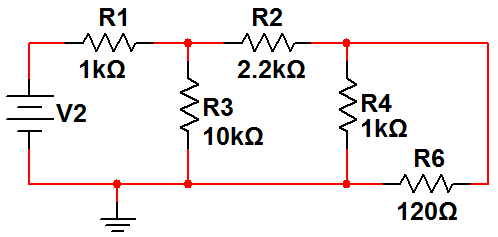
\includegraphics[scale=0.5]{c2.png}
	\caption{Fuente $V_1$ a cero}
	\label{fig3}
\end{figure}
\noindent
Las ecuaciones para este circuito son las siguientes:
\begin{equation}
 {V_2} = {I_{1b}}\left( {{R_1} + {R_3}} \right) - {I_{2b}}{R_3}
\end{equation}
\begin{equation}
 0 =  - {I_-{1b}}{R_3} + {I_{2b}}\left( {{R_2} + {R_3} + {R_4}} \right) - {I_{3b}}{R_4}
\end{equation}
\begin{equation}
 0 =  - {I_{2b}}{R_4} + {I_{3b}}\left( {{R_4} + {R_5} + {R_6}} \right)
\end{equation}
\noindent
En forma matricial
\begin{equation}
\footnotesize
 \left[ {\begin{array}{*{20}{c}}
   {{R_1} + {R_3}} & { - {R_3}} & 0  \\
   {{R_3}} & {{R_2} + {R_3} + {R_4}} & { - {R_4}}  \\
   0 & { - {R_4}} & {{R_4} + {R_5} + {R_6}}  \\
\end{array}} \right]\left[ \begin{array}{l}
 {I_{1b}} \\ 
 {I_{2b}} \\ 
 {I_{3b}} \\ 
 \end{array} \right] = \left[ \begin{array}{l}
 {V_2} \\ 
 0 \\ 
 0 \\ 
 \end{array} \right]
\label{mat3}
\end{equation}
\begin{equation}
\footnotesize
 \left[ \begin{array}{l}
 {I_{1b}} \\ 
 {I_{2b}} \\ 
 {I_{3b}} \\ 
 \end{array} \right] = {\left[ {\begin{array}{*{20}{c}}
   {{R_1} + {R_3}} & { - {R_3}} & 0  \\
   {{R_3}} & {{R_2} + {R_3} + {R_4}} & { - {R_4}}  \\
   0 & { - {R_4}} & {{R_4} + {R_5} + {R_6}}  \\
\end{array}} \right]^{ - 1}}\left[ \begin{array}{l}
 {V_2} \\ 
 0 \\ 
 0 \\ 
 \end{array} \right]
\label{mat4}
\end{equation}
El valor de las corrientes para el circuito \ref{fig3} se encuentran a continuación
\begin{equation}
 \left[ \begin{array}{l}
 {I_{1b}} \\ 
 {I_{2b}} \\ 
 {I_{3}} \\ 
 \end{array} \right] = \left[ \begin{array}{l}
 8.553 \ mA \\ 
 6.909 \ mA \\ 
 5.663 \ mA \\ 
 \end{array} \right]
\end{equation}
\noindent
El valor de las corrientes es el siguiente
\begin{equation}
\footnotesize
 \left[ \begin{array}{l}
 {I_{1a}} \\ 
 {I_{2a}} \\ 
 {I_{3a}} \\ 
 {I_{4a}} \\ 
 \end{array} \right] + \left[ \begin{array}{l}
 {I_{1b}} \\ 
 {I_{2b}} \\ 
 {I_{3b}} \\ 
 {I_{4b}} \\ 
 \end{array} \right] = \left[ \begin{array}{l}
 1.132 \\ 
 1.245 \\ 
 5.119 \\ 
 0.05 \\ 
 \end{array} \right] + \left[ \begin{array}{l}
 8.553 \\ 
 6.909 \\ 
 5.663 \\ 
 0 \\ 
 \end{array} \right] = \left[ \begin{array}{l}
 9.685 \ mA \\ 
 8.154 \ mA \\ 
 10.782 \ mA \\ 
 0.05 \ mA \\ 
 \end{array} \right]
\end{equation}

\section{Circuito con 2 fuentes de voltaje}
\noindent
Se calculo los resultados teóricos del circuito de la Fig. \ref{fig4}
\begin{figure}[H]
	\centering
		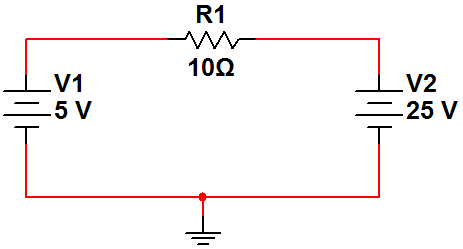
\includegraphics[scale=0.5]{c3.png}
	\caption{Montaje con $2$ fuentes}
	\label{fig4}
\end{figure}
\noindent
Las ecuaciones que se obtuvieron se describen a continuación
\begin{equation}
{V_1} - {V_2} = I \ R
\end{equation}
\begin{equation}
 \frac{{V_1} - {V_2}}{R}
\end{equation}
\noindent
Es decir que el valor de la corriente es $\frac{5 - 10}{10} = -0.5\ A$, esto quiere decir que el voltaje en la resistencia es de $5\ V$ y la fuente $V_1$ esta consumiendo corriente y energía

\section{Preguntas}
\begin{enumerate}
 \item ¿En la teoría existen diferencias entre los valores obtenidos con nodos y los obtenidos
con mallas?\\
Gracias a que las teorías de nodos y de mallas se derivan de la ley  Ohm y las ecuaciones de Maxwell los datos que se obtienen a través de estas  no tienen diferencia.
 \item ¿Existen diferencias entre los valores obtenidos en la teoría y los valores experimentales?\\
En la teoría se asumen que los elementos del circuito son ideales, es decir que las fuentes y generador de señales no tienen pérdidas internas, que no hay pérdidas en los cables y las resistencias tienen valores exactos. Ahora experimentalmente se tienen estas clases de pérdidas tanto en fuentes, en generadores de señales  como en cables de conexiones, además los valores de resistencias no son exactos y los elementos de medición pueden no medir con precisión y exactitud.\\
Pero aun así, los valores tomados experimentalmente generalmente se aproximan a los datos obtenidos teóricamente.
 \item ¿En la práctica para realizar superposición, es lo mismo poner la fuente DC o el generador de señales en cero voltios que ponerlos en corto?  Concuerda con la teoría?\\
Cuando se pone una fuente DC o un generador de señales en cero voltios, este representa una resistencia interna considerable la cual modifica el análisis del circuito, el cual se comporta diferente si en lugar de la fuente o el generador de señales  se pone en corto ya que representa una resistencia aproximadamente de  cero.\\
Esto no concuerda con la teoría, ya que en esta es lo mismo dejar la fuente o el generador de señales en cero voltios o ponerlos en corto, en las ecuaciones de análisis esto no alterara el resultado.
 \item ¿Hay diferencias en la curva ($V \ vs \ I$) de una fuente real y una teórica?\\
Suponiendo que se analiza un circuito lineal, la curva de una fuente ideal es lineal, con la corriente proporcional a la tensión ya que esta fuente puede entregar la corriente que pida el circuito. En una fuente real la curva no es lineal ya que está limitada por corriente, al acercarse al límite  o alcanzarlo se puede calentar y la resistencia interna de la fuente aumenta. 
 \item ¿Cual será el modelo adecuado para la fuente de tensión DC y para el generador de señales?
La fuente de tensión real se modela adecuadamente como una fuente de tensión ideal con una resistencia en serie, esta resistencia representa la resistencia interna de la fuente. El generador de señales se modela de igual forma, con una fuente AC ideal  con una resistencia en serie.
\begin{figure}[H]
	\centering
		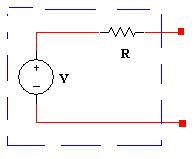
\includegraphics[scale=0.9]{p1.png}
	\caption{Modelo para una fuente de tensión real}
	\label{fig10}
\end{figure}
\begin{figure}[H]
	\centering
		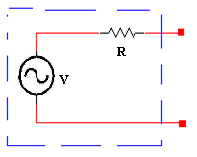
\includegraphics[scale=0.9]{p11.png}
	\caption{Modelo para una generador de señales real}
	\label{fig11}
\end{figure}

 \item ¿En qué casos es conveniente usar superposición para análisis de circuitos?\\
La superposición se usa cuando se tienen dos o más fuentes que afectan a un elemento del circuito, pero más conveniente usar este método de análisis cuando se tiene que estas fuentes son AC con la misma o diferente frecuencia, cuando son fuentes AC con un nivel DC o combinación de estas.
\end{enumerate}

\bibliographystyle{ieeetran}
\begin{thebibliography}{99}
\bibitem{dorf} Dorf  \& Svoboda.
{\em "`Circuitos Eléctricos"'}.
Alfaomega, Sexta Edición, 2006.

\bibitem{sadiku} Alexander, Charles K. \&  Sadiku, Matthew N.O.
{\em "`Fundamentals of Electric Circuits"'}.
McGRAW-HILL, ISE Editions, 1999.

\bibitem{nahvi} Nahvi, Mahmood \& Edminister, Joseph A.
{\em "`Theory and Problems of Electric Circuits"'}.
McGRAW-HILL, Fourth Edition, 2003.
\end{thebibliography}
\end{document}
